% Created by tikzDevice version 0.12
% !TEX encoding = UTF-8 Unicode
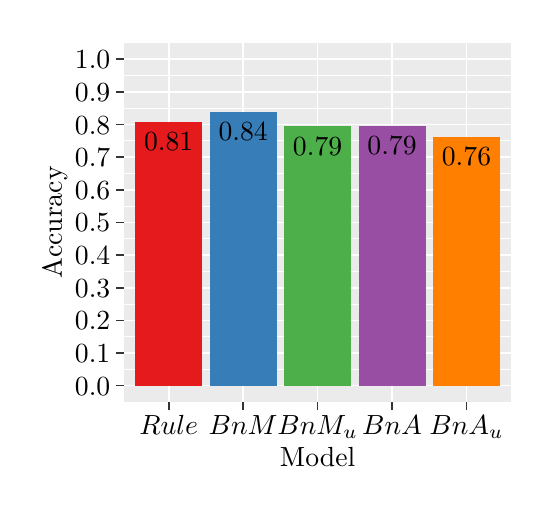
\begin{tikzpicture}[x=1pt,y=1pt]
\definecolor{fillColor}{RGB}{255,255,255}
\path[use as bounding box,fill=fillColor,fill opacity=0.00] (0,0) rectangle (180.22,166.12);
\begin{scope}
\path[clip] (  0.00,  0.00) rectangle (180.22,166.12);
\definecolor{drawColor}{RGB}{255,255,255}
\definecolor{fillColor}{RGB}{255,255,255}

\path[draw=drawColor,line width= 0.6pt,line join=round,line cap=round,fill=fillColor] (  0.00,  0.00) rectangle (180.22,166.12);
\end{scope}
\begin{scope}
\path[clip] ( 34.81, 30.86) rectangle (174.72,160.62);
\definecolor{fillColor}{gray}{0.92}

\path[fill=fillColor] ( 34.81, 30.86) rectangle (174.72,160.62);
\definecolor{drawColor}{RGB}{255,255,255}

\path[draw=drawColor,line width= 0.3pt,line join=round] ( 34.81, 42.66) --
	(174.72, 42.66);

\path[draw=drawColor,line width= 0.3pt,line join=round] ( 34.81, 54.45) --
	(174.72, 54.45);

\path[draw=drawColor,line width= 0.3pt,line join=round] ( 34.81, 66.25) --
	(174.72, 66.25);

\path[draw=drawColor,line width= 0.3pt,line join=round] ( 34.81, 78.05) --
	(174.72, 78.05);

\path[draw=drawColor,line width= 0.3pt,line join=round] ( 34.81, 89.84) --
	(174.72, 89.84);

\path[draw=drawColor,line width= 0.3pt,line join=round] ( 34.81,101.64) --
	(174.72,101.64);

\path[draw=drawColor,line width= 0.3pt,line join=round] ( 34.81,113.43) --
	(174.72,113.43);

\path[draw=drawColor,line width= 0.3pt,line join=round] ( 34.81,125.23) --
	(174.72,125.23);

\path[draw=drawColor,line width= 0.3pt,line join=round] ( 34.81,137.03) --
	(174.72,137.03);

\path[draw=drawColor,line width= 0.3pt,line join=round] ( 34.81,148.82) --
	(174.72,148.82);

\path[draw=drawColor,line width= 0.6pt,line join=round] ( 34.81, 36.76) --
	(174.72, 36.76);

\path[draw=drawColor,line width= 0.6pt,line join=round] ( 34.81, 48.56) --
	(174.72, 48.56);

\path[draw=drawColor,line width= 0.6pt,line join=round] ( 34.81, 60.35) --
	(174.72, 60.35);

\path[draw=drawColor,line width= 0.6pt,line join=round] ( 34.81, 72.15) --
	(174.72, 72.15);

\path[draw=drawColor,line width= 0.6pt,line join=round] ( 34.81, 83.94) --
	(174.72, 83.94);

\path[draw=drawColor,line width= 0.6pt,line join=round] ( 34.81, 95.74) --
	(174.72, 95.74);

\path[draw=drawColor,line width= 0.6pt,line join=round] ( 34.81,107.54) --
	(174.72,107.54);

\path[draw=drawColor,line width= 0.6pt,line join=round] ( 34.81,119.33) --
	(174.72,119.33);

\path[draw=drawColor,line width= 0.6pt,line join=round] ( 34.81,131.13) --
	(174.72,131.13);

\path[draw=drawColor,line width= 0.6pt,line join=round] ( 34.81,142.92) --
	(174.72,142.92);

\path[draw=drawColor,line width= 0.6pt,line join=round] ( 34.81,154.72) --
	(174.72,154.72);

\path[draw=drawColor,line width= 0.6pt,line join=round] ( 50.95, 30.86) --
	( 50.95,160.62);

\path[draw=drawColor,line width= 0.6pt,line join=round] ( 77.86, 30.86) --
	( 77.86,160.62);

\path[draw=drawColor,line width= 0.6pt,line join=round] (104.76, 30.86) --
	(104.76,160.62);

\path[draw=drawColor,line width= 0.6pt,line join=round] (131.67, 30.86) --
	(131.67,160.62);

\path[draw=drawColor,line width= 0.6pt,line join=round] (158.57, 30.86) --
	(158.57,160.62);
\definecolor{fillColor}{RGB}{228,26,28}

\path[fill=fillColor] ( 38.84, 36.76) rectangle ( 63.06,132.03);
\definecolor{fillColor}{RGB}{55,126,184}

\path[fill=fillColor] ( 65.75, 36.76) rectangle ( 89.96,135.79);
\definecolor{fillColor}{RGB}{77,175,74}

\path[fill=fillColor] ( 92.65, 36.76) rectangle (116.87,130.45);
\definecolor{fillColor}{RGB}{152,78,163}

\path[fill=fillColor] (119.56, 36.76) rectangle (143.78,130.52);
\definecolor{fillColor}{RGB}{255,127,0}

\path[fill=fillColor] (146.47, 36.76) rectangle (170.68,126.51);
\definecolor{drawColor}{RGB}{0,0,0}

\node[text=drawColor,anchor=base,inner sep=0pt, outer sep=0pt, scale=  1.00] at (158.57,116.14) {0.76};

\node[text=drawColor,anchor=base,inner sep=0pt, outer sep=0pt, scale=  1.00] at (131.67,120.14) {0.79};

\node[text=drawColor,anchor=base,inner sep=0pt, outer sep=0pt, scale=  1.00] at (104.76,120.07) {0.79};

\node[text=drawColor,anchor=base,inner sep=0pt, outer sep=0pt, scale=  1.00] at ( 77.86,125.42) {0.84};

\node[text=drawColor,anchor=base,inner sep=0pt, outer sep=0pt, scale=  1.00] at ( 50.95,121.66) {0.81};
\end{scope}
\begin{scope}
\path[clip] (  0.00,  0.00) rectangle (180.22,166.12);
\definecolor{drawColor}{RGB}{0,0,0}

\node[text=drawColor,anchor=base east,inner sep=0pt, outer sep=0pt, scale=  1.00] at ( 29.86, 33.32) {0.0};

\node[text=drawColor,anchor=base east,inner sep=0pt, outer sep=0pt, scale=  1.00] at ( 29.86, 45.11) {0.1};

\node[text=drawColor,anchor=base east,inner sep=0pt, outer sep=0pt, scale=  1.00] at ( 29.86, 56.91) {0.2};

\node[text=drawColor,anchor=base east,inner sep=0pt, outer sep=0pt, scale=  1.00] at ( 29.86, 68.70) {0.3};

\node[text=drawColor,anchor=base east,inner sep=0pt, outer sep=0pt, scale=  1.00] at ( 29.86, 80.50) {0.4};

\node[text=drawColor,anchor=base east,inner sep=0pt, outer sep=0pt, scale=  1.00] at ( 29.86, 92.30) {0.5};

\node[text=drawColor,anchor=base east,inner sep=0pt, outer sep=0pt, scale=  1.00] at ( 29.86,104.09) {0.6};

\node[text=drawColor,anchor=base east,inner sep=0pt, outer sep=0pt, scale=  1.00] at ( 29.86,115.89) {0.7};

\node[text=drawColor,anchor=base east,inner sep=0pt, outer sep=0pt, scale=  1.00] at ( 29.86,127.68) {0.8};

\node[text=drawColor,anchor=base east,inner sep=0pt, outer sep=0pt, scale=  1.00] at ( 29.86,139.48) {0.9};

\node[text=drawColor,anchor=base east,inner sep=0pt, outer sep=0pt, scale=  1.00] at ( 29.86,151.28) {1.0};
\end{scope}
\begin{scope}
\path[clip] (  0.00,  0.00) rectangle (180.22,166.12);
\definecolor{drawColor}{gray}{0.20}

\path[draw=drawColor,line width= 0.6pt,line join=round] ( 32.06, 36.76) --
	( 34.81, 36.76);

\path[draw=drawColor,line width= 0.6pt,line join=round] ( 32.06, 48.56) --
	( 34.81, 48.56);

\path[draw=drawColor,line width= 0.6pt,line join=round] ( 32.06, 60.35) --
	( 34.81, 60.35);

\path[draw=drawColor,line width= 0.6pt,line join=round] ( 32.06, 72.15) --
	( 34.81, 72.15);

\path[draw=drawColor,line width= 0.6pt,line join=round] ( 32.06, 83.94) --
	( 34.81, 83.94);

\path[draw=drawColor,line width= 0.6pt,line join=round] ( 32.06, 95.74) --
	( 34.81, 95.74);

\path[draw=drawColor,line width= 0.6pt,line join=round] ( 32.06,107.54) --
	( 34.81,107.54);

\path[draw=drawColor,line width= 0.6pt,line join=round] ( 32.06,119.33) --
	( 34.81,119.33);

\path[draw=drawColor,line width= 0.6pt,line join=round] ( 32.06,131.13) --
	( 34.81,131.13);

\path[draw=drawColor,line width= 0.6pt,line join=round] ( 32.06,142.92) --
	( 34.81,142.92);

\path[draw=drawColor,line width= 0.6pt,line join=round] ( 32.06,154.72) --
	( 34.81,154.72);
\end{scope}
\begin{scope}
\path[clip] (  0.00,  0.00) rectangle (180.22,166.12);
\definecolor{drawColor}{gray}{0.20}

\path[draw=drawColor,line width= 0.6pt,line join=round] ( 50.95, 28.11) --
	( 50.95, 30.86);

\path[draw=drawColor,line width= 0.6pt,line join=round] ( 77.86, 28.11) --
	( 77.86, 30.86);

\path[draw=drawColor,line width= 0.6pt,line join=round] (104.76, 28.11) --
	(104.76, 30.86);

\path[draw=drawColor,line width= 0.6pt,line join=round] (131.67, 28.11) --
	(131.67, 30.86);

\path[draw=drawColor,line width= 0.6pt,line join=round] (158.57, 28.11) --
	(158.57, 30.86);
\end{scope}
\begin{scope}
\path[clip] (  0.00,  0.00) rectangle (180.22,166.12);
\definecolor{drawColor}{RGB}{0,0,0}

\node[text=drawColor,anchor=base,inner sep=0pt, outer sep=0pt, scale=  1.00] at ( 50.95, 19.03) {\(Rule\)};

\node[text=drawColor,anchor=base,inner sep=0pt, outer sep=0pt, scale=  1.00] at ( 77.86, 19.03) {\(BnM\)};

\node[text=drawColor,anchor=base,inner sep=0pt, outer sep=0pt, scale=  1.00] at (104.76, 19.03) {\(BnM_u\)};

\node[text=drawColor,anchor=base,inner sep=0pt, outer sep=0pt, scale=  1.00] at (131.67, 19.03) {\(BnA\)};

\node[text=drawColor,anchor=base,inner sep=0pt, outer sep=0pt, scale=  1.00] at (158.57, 19.03) {\(BnA_u\)};
\end{scope}
\begin{scope}
\path[clip] (  0.00,  0.00) rectangle (180.22,166.12);
\definecolor{drawColor}{RGB}{0,0,0}

\node[text=drawColor,anchor=base,inner sep=0pt, outer sep=0pt, scale=  1.00] at (104.76,  7.44) {Model};
\end{scope}
\begin{scope}
\path[clip] (  0.00,  0.00) rectangle (180.22,166.12);
\definecolor{drawColor}{RGB}{0,0,0}

\node[text=drawColor,rotate= 90.00,anchor=base,inner sep=0pt, outer sep=0pt, scale=  1.00] at ( 12.39, 95.74) {Accuracy};
\end{scope}
\end{tikzpicture}
